\section{Simulation 2: Two-Layer Neural Network}
\label{sec:simulation2}

\subsection{Data and Hyperparameters}

We generated balanced noisy semicircles. For each example, we sampled an independent
angle $t\sim\operatorname{Uniform}[0,\pi]$ and input perturbation
$e\sim\mathcal{N}(0,0.1^2I_2)$, then constructed
\[
a=\begin{cases}
(\cos t,\sin t)^\top+e,&y=0,\\
(1-\cos t,\tfrac12-\sin t)^\top+e,&y=1.
\end{cases}
\]
We used 1,000 training, 400 validation, and 400 test examples. The dataset seed
was 42, with seeds 43 and 44 for the validation and test splits.
All runs used these same three datasets. We applied no input preprocessing.

The network was
\[
t_\theta(a)=w_2^\top\tanh(W_1a+b_1)+b_2,
\qquad W_1\in\mathbb{R}^{8\times2},
\]
with 33 trainable parameters. We initialized both weight matrices with
Xavier-uniform initialization, using the tanh gain in the hidden layer,
and initialized biases to zero. Paired runs used identical initial parameters.
We minimized mean binary cross-entropy from logits, without weight decay or an
additional loss regularizer, and classified at logit zero.
The per-example automatic derivatives were checked against central finite
differences for all 33 parameters in float64.

The initial learning-rate and radius grids were
\[
\alpha_0\in\{0.01,0.1,1,3,10,100\},\qquad
\rho\in\{0,0.1,0.3,1,3\}.
\]
The training seeds were 1 through 15.
Fixed hyperparameters:
\begin{itemize}
    \item $\texttt{batch\_size}=32$, sampled independently with replacement;
    \item $\texttt{updates}=500$;
    \item $\texttt{decay\_scale}=50$;
    \item $\texttt{eval\_every}=25$;
    \item learning-rate schedule $\alpha_k=\alpha_0/\sqrt{1+k/50}$, starting at $k=0$.
\end{itemize}
Each run therefore used $32\times500=16{,}000$ per-example gradient observations.
Initial learning rate and radius were selected using mean final clean validation
loss across the 15 seeds. Test metrics did not enter selection.

\paragraph{Execution environment.}
The repeat used an Apple M4 Pro MacBook Pro (Mac16,8), with 12 CPU cores
(8 performance and 4 efficiency), 24 GiB unified memory, and an internal Apple
512 GB SSD. The integrated 16-core GPU was unused.
Training ran in CPU float32 with eight worker processes and one PyTorch
intra-operation thread per worker. The environment used Python 3.12.14,
PyTorch 2.15.0, and macOS 26.6.2. Timings include concurrent CPU contention.
Power, temperature, peak memory, and clock frequencies were not measured.

\subsection{Grid Search}
\label{sec:sim2_search}

We searched the following initial learning rates and robustness radii:
\[
\alpha_0\in\{0.01,0.1,1,3,10,100\},
\qquad
\rho\in\{0,0.1,0.3,1,3\}.
\]
For SGD, only $\alpha_0$ was varied, with $\rho=0$.
For R-SGD, every LR--radius combination was evaluated, including $\rho=0$.
Each configuration was trained with seeds 1 through 15.

The unrestricted search selected $\alpha_0=10$ and $\rho=0$ for both methods.
Thus, the lowest mean clean validation loss in the tested grid was achieved by
ordinary SGD. To examine a positive robustness radius, we also selected the
best point subject to $\rho>0$. This gave $\alpha_0=10$ and $\rho=1$.
The SGD and positive-radius R-SGD settings were then frozen for the noise sweep.

\begin{table}[htbp]
\centering
\begin{tabular}{lrrr}
\toprule
Comparison & Initial LR & Radius & Mean validation BCE\\
\midrule
SGD / unrestricted winner & 10 & 0 & 0.003219\\
Best positive-radius R-SGD & 10 & 1 & 0.004569\\
\bottomrule
\end{tabular}
\caption{Simulation 2 settings selected using clean validation loss.}
\label{tab:sim2_selection}
\end{table}

Neither selected initial learning rate was at an endpoint of the tested range,
and the selected positive radius was also interior to its range.
The unrestricted radius was at the lower endpoint, $\rho=0$.
We ran 90 SGD tuning runs and 450 runs in the LR--radius grid,
including an additional $\rho=0$ baseline, for 540 tuning runs in total.
Figure~\ref{fig:sim2_tuning} shows the validation-loss surface.

\subsection{Experiments with Noisy Gradients}
\label{sec:sim2_noise}

We perturbed each per-example gradient independently using the isotropic
Gaussian model described in Section~\ref{sec:general_setup}.
The original protocol calibrated a shared scale using 50 clean warmup updates
per seed at the unrestricted winner ($\alpha_0=10$, $\rho=0$).
The scale was $\sigma_{\mathrm{scale}}=0.17038964$.
We retained that calibration for the positive-radius comparison, giving
\[
\sigma\in\{0,\ 0.01703896,\ 0.05111689,\ 0.17038964,\ 0.42597409\}.
\]
Both methods used the same absolute noise levels and matched random streams
for initialization, replacement sampling, and gradient perturbations.
The gradient mean and diagonal uncertainty matrix were constructed from the
perturbed observations actually used by the optimizer.
The objective and evaluation data received no artificial gradient perturbations.

Figure~\ref{fig:sim2_loss_curves} shows training and validation losses at all five
noise levels. Figure~\ref{fig:sim2_boundary} shows the decision boundaries for
evaluation seed 1. Final losses and accuracies are summarized below and in
Figure~\ref{fig:sim2_metrics}.

\begin{table}[htbp]
\centering
\small
\begin{tabular}{rlrrrr}
\toprule
$\sigma$ & Method & Train BCE & Test BCE & Test accuracy (\%) & Runtime (s)\\
\midrule
0       & SGD   & 0.00349 & 0.00472 & 99.833 & 0.252\\
0       & R-SGD & 0.00680 & 0.00637 & 99.833 & 0.657\\
0.01704 & SGD   & 0.00407 & 0.00433 & 99.867 & 0.263\\
0.01704 & R-SGD & 0.00829 & 0.00669 & 99.817 & 0.682\\
0.05112 & SGD   & 0.00373 & 0.00414 & 99.867 & 0.258\\
0.05112 & R-SGD & 0.00906 & 0.00836 & 99.767 & 0.680\\
0.17039 & SGD   & 0.00935 & 0.01056 & 99.700 & 0.258\\
0.17039 & R-SGD & 0.01560 & 0.01235 & 99.583 & 0.658\\
0.42597 & SGD   & 0.02938 & 0.02612 & 99.500 & 0.264\\
0.42597 & R-SGD & 0.03280 & 0.02703 & 99.167 & 0.651\\
\bottomrule
\end{tabular}
\caption{Simulation 2 means across 15 seeds. All selected-setting runs used
16,000 gradient observations and had zero-step frequency zero.
Runtime covers the full training loop, including periodic evaluation.
Figure~\ref{fig:sim2_metrics} shows one-sample-standard-deviation error bars.}
\label{tab:sim2_metrics}
\end{table}

\begin{itemize}
    \item SGD achieved lower mean training and test BCE at every noise level.
    Clean test accuracy was equal at 99.833\%, despite different training losses.
    At the highest noise level, test accuracy was 99.500\% for SGD and
    99.167\% for R-SGD. This dataset leaves little room for accuracy gains.
    \item Paired results reveal variation hidden by the means. At
    $\sigma=0.17039$ and $0.42597$, R-SGD achieved lower test BCE in
    10 of 15 and 9 of 15 seeds, respectively. Its worse runs outweighed these
    improvements in the arithmetic mean. These counts describe this sample of
    seeds and provide no significance test.
    \item Every selected R-SGD run had zero-step frequency zero. A nonzero
    robust update can still be shorter and have a different direction from
    the corresponding SGD update. Complete stops therefore provide only one
    diagnostic of robust behavior.
    \item The robust solver increased the measured training runtime.
    Paired runs had equal gradient budgets. Concurrent worker contention and
    the use of the same gradient-observation pipeline for both methods limit
    the interpretation of wall-clock ratios.
\end{itemize}

\subsection{Sensitivity to Robustness Radius}
\label{sec:sim2_radius}

Figure~\ref{fig:sim2_radius} varies $\rho$ at fixed $\alpha_0=10$, with a separate
curve for every noise level. Each point averages 15 seeds.
The clean mean validation BCE at radii
$0$, $0.1$, $0.3$, $1$, and $3$ was approximately
$0.00322$, $0.02315$, $0.00519$, $0.00457$, and $0.02528$.
The observed relationship was nonmonotonic. Larger radius did not uniformly
improve the result.

For clean gradients, mean zero-step frequency increased from zero at
$\rho\leq1$ to 1.8\% at $\rho=3$. This follows the stopping condition
\[
g_k^\top S_k^{-1}g_k\leq\rho^2.
\]
Along different training trajectories, both $g_k$ and $S_k$ change, so monotonic
frequency across trained runs is not guaranteed by this condition.
In this study, stops were too infrequent to produce the large runtime decrease
seen in Simulation 1. Positive-radius runs still required the scalar solver on
most updates.

The added perturbations were isotropic, but the covariance of the observed
gradients also contains the covariance of the clean per-example gradients.
Conditionally on the current parameters,
\[
\operatorname{Cov}(g_k)
=\frac{1}{b}\left(\operatorname{Cov}_i[u_i(\theta_k)]+\sigma^2I\right).
\]
Consequently, isotropic added noise alone does not imply $S_k=sI$.
The isotropic closed-form shrinkage interpretation applies when the
uncertainty matrix itself is isotropic. Step-length and direction effects
were not isolated by these outcome plots.

\subsection{Reproducibility and Limitations}
\label{sec:sim2_reproducibility}

All 990 runs completed without failure, comprising 540 tuning runs and 450
noise/radius evaluations. Calibration added 750 updates.
The overall budget was 495,750 updates and 15,864,000 per-example gradient
observations. Each of the 450 saved evaluation histories has 21 records,
from update 0 through update 500. Repeated losses and accuracies matched the
original study.

The report assets include the selected settings, the aggregate noise and tuning
tables, and the plotting manifest. All figures use linear axes.
Shading and error bars denote one sample standard deviation across the 15
training seeds. They describe training randomness on this fixed dataset.
They do not estimate variability across newly generated datasets.

The same training seeds were used for tuning and evaluation. A focused next
experiment would freeze these configurations and compare them on fresh paired
training seeds, reporting paired loss differences. A separate study over new
dataset seeds would assess sensitivity to the sampled dataset.
Within the present experiment, R-SGD provided no consistent average advantage
over SGD at the chosen positive radius.

\clearpage
\begin{figure}[p]
    \centering
    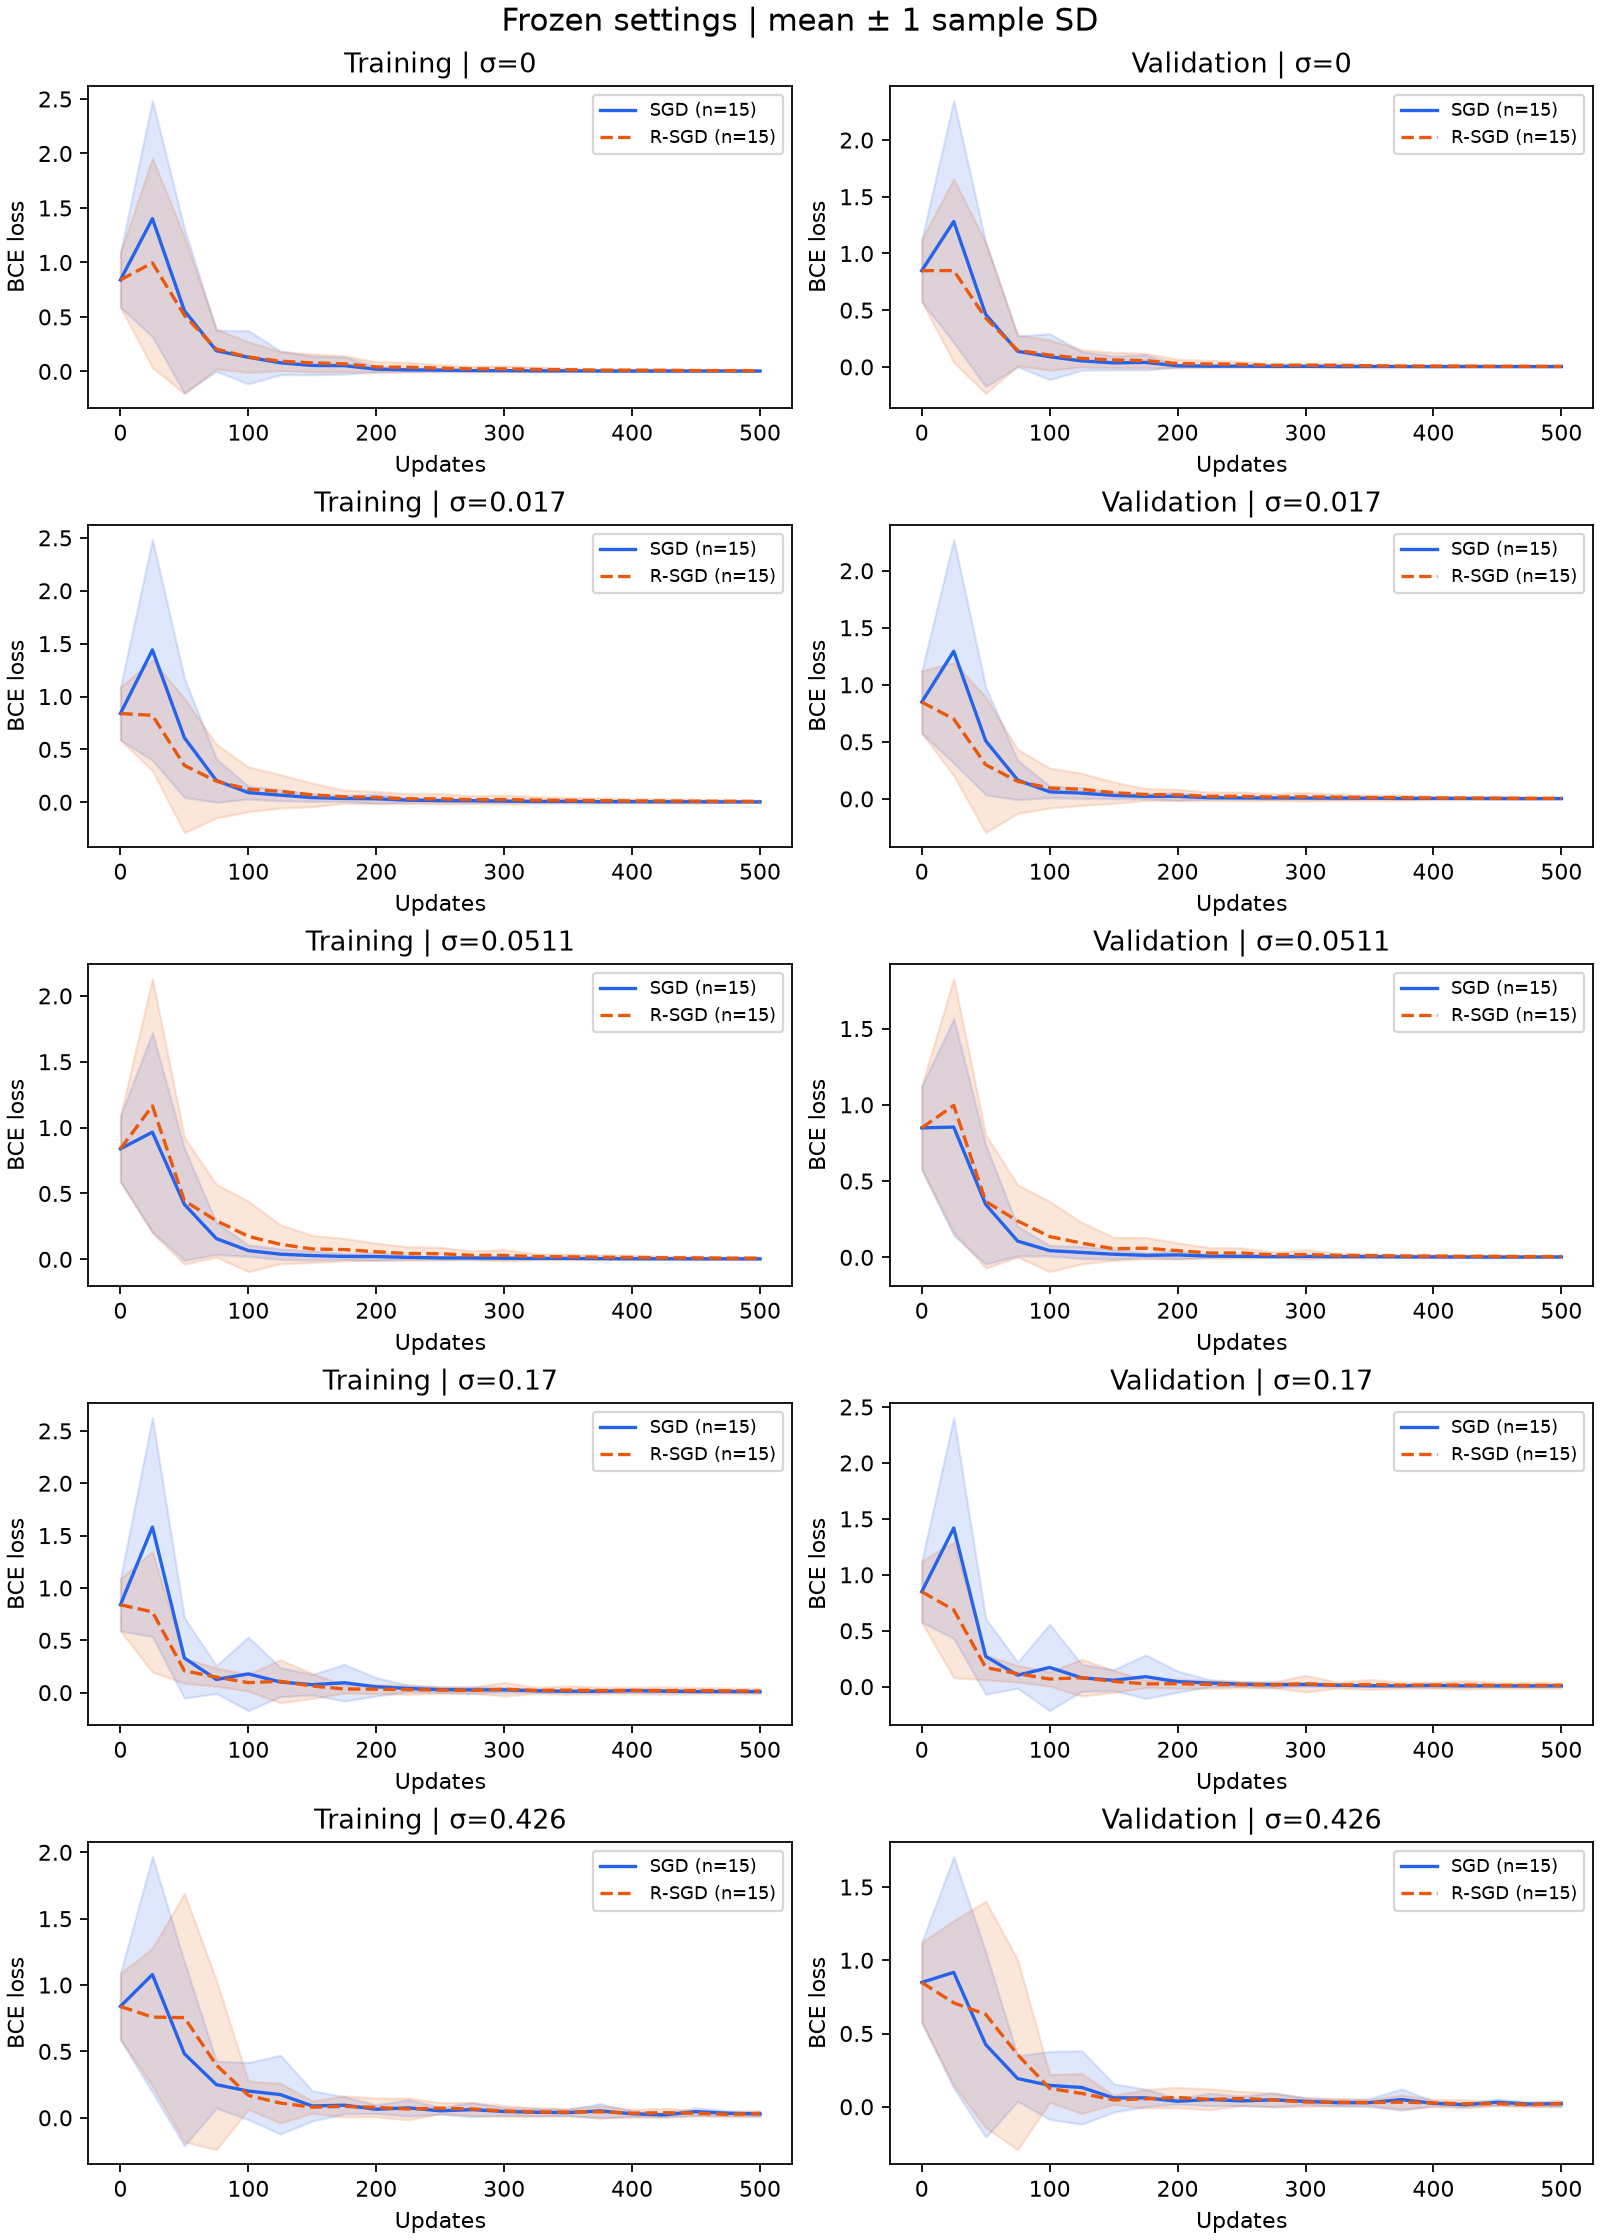
\includegraphics[width=0.9\textwidth,height=0.82\textheight,keepaspectratio]{./plots/semicircle/loss_curves.png}
    \caption{Simulation 2 training and validation BCE against updates at all five
    noise levels. SGD uses LR 10 and radius 0. R-SGD uses LR 10 and radius 1.
    Curves are means, with one-sample-standard-deviation bands across 15 seeds.
    Negative band endpoints arise from the arithmetic mean-minus-SD summary,
    while every observed BCE is nonnegative.}
    \label{fig:sim2_loss_curves}
\end{figure}

\begin{figure}[p]
    \centering
    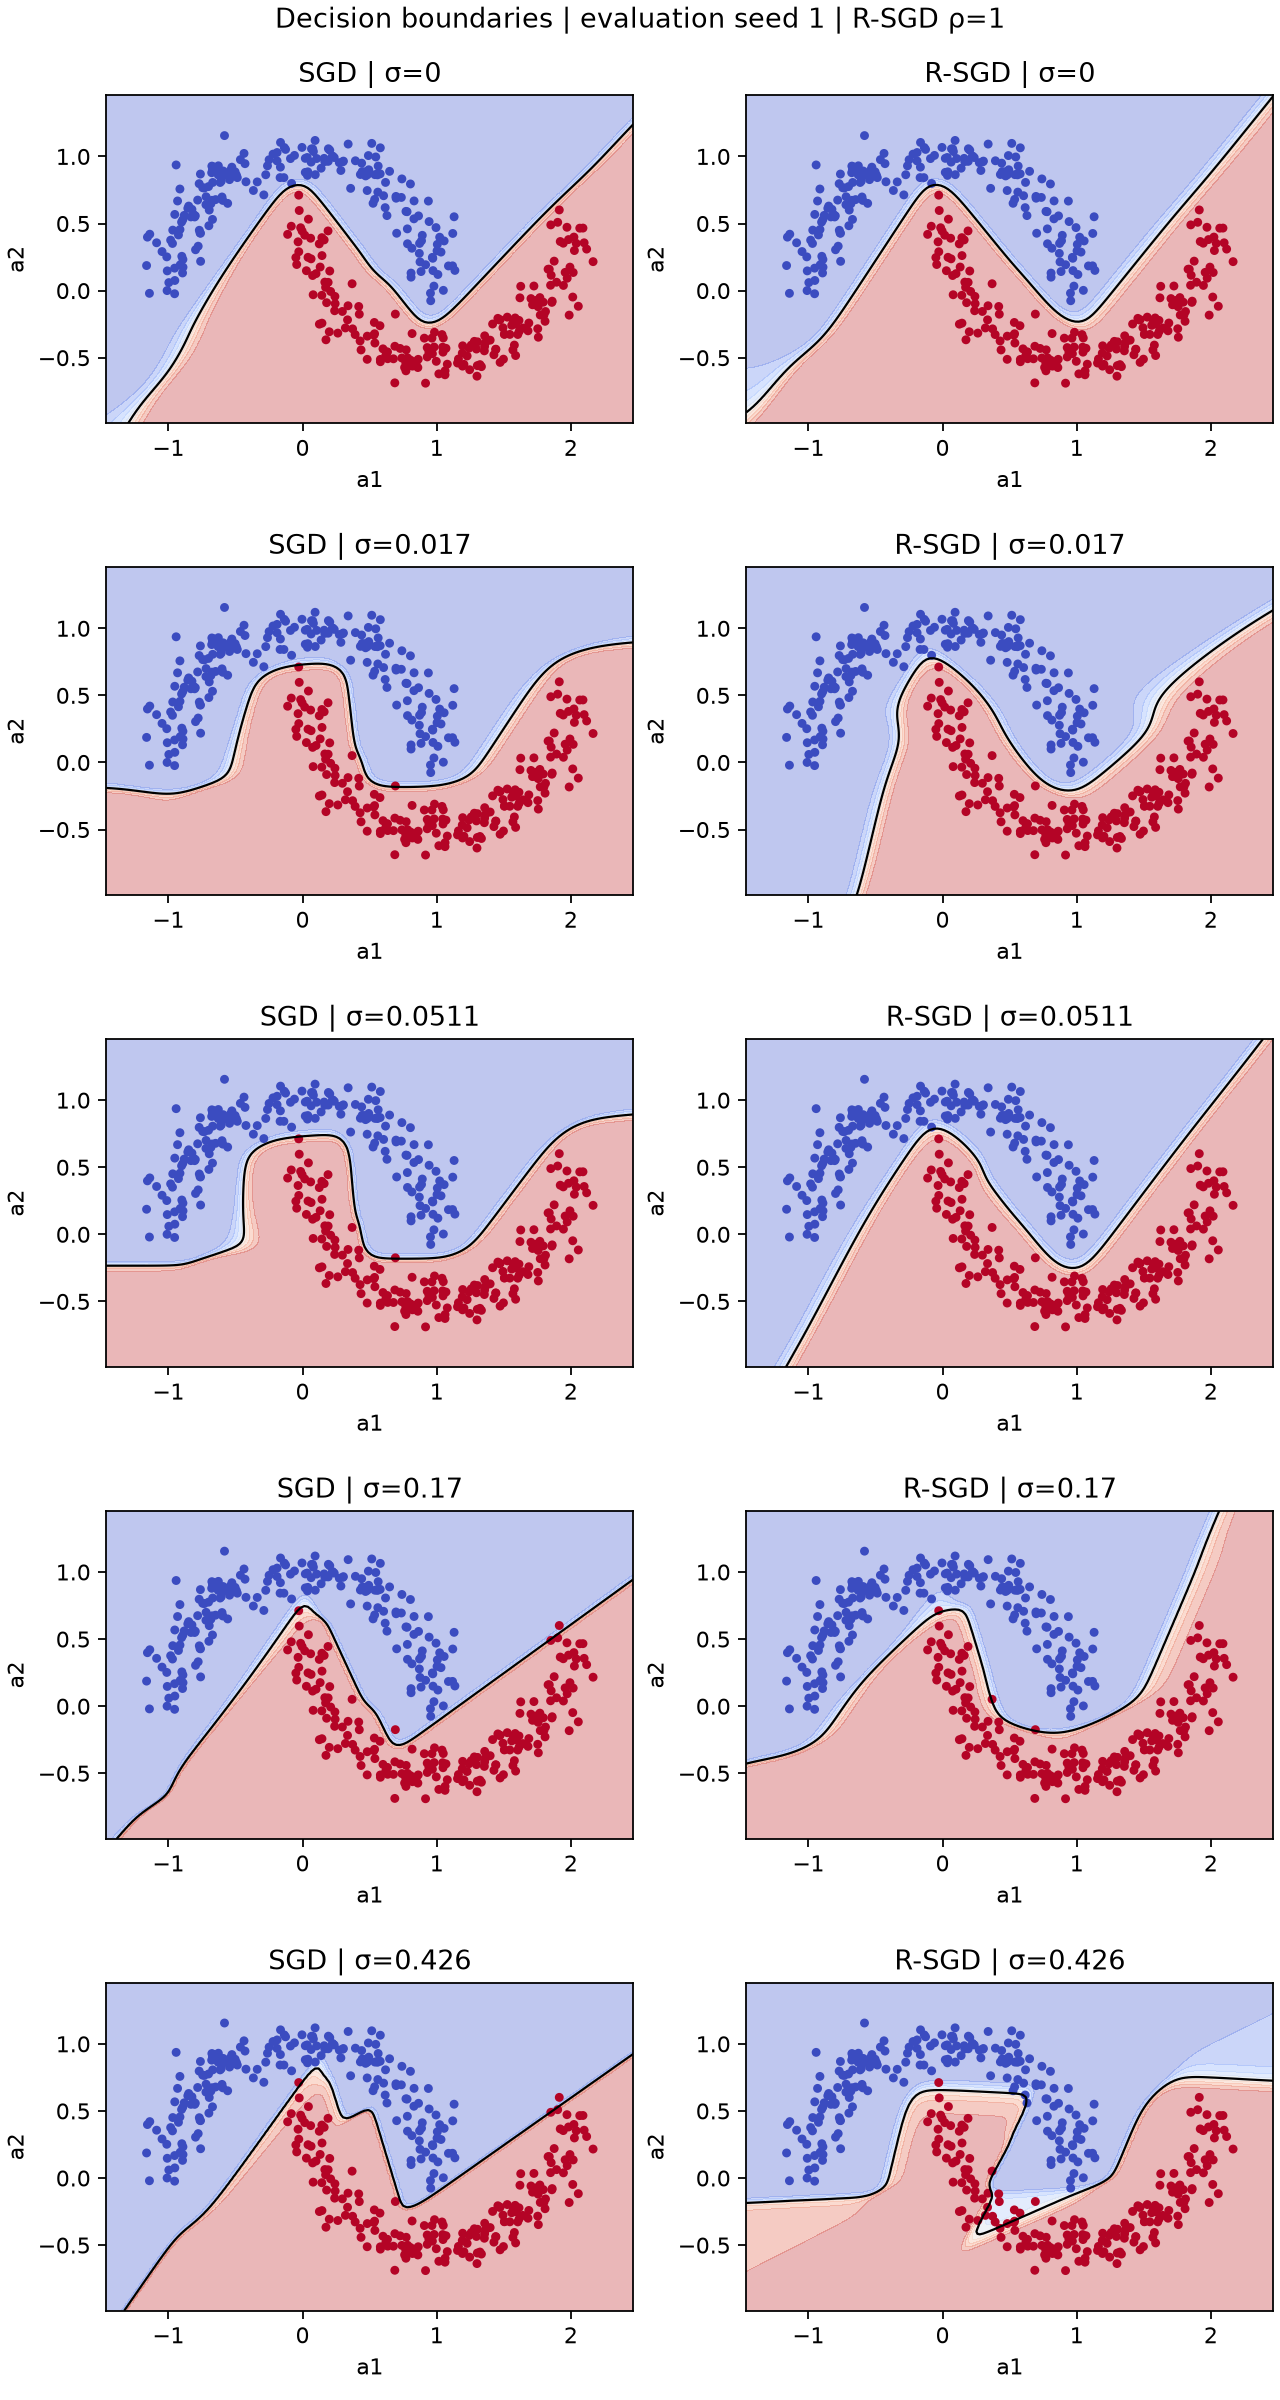
\includegraphics[width=0.95\textwidth,height=0.82\textheight,keepaspectratio]{./plots/semicircle/decision_boundaries.png}
    \caption{Simulation 2 decision boundaries for evaluation seed 1 on the fixed
    clean test set. Rows vary gradient noise and columns compare SGD with
    positive-radius R-SGD. Black contours mark logit zero.}
    \label{fig:sim2_boundary}
\end{figure}

\begin{figure}[p]
    \centering
    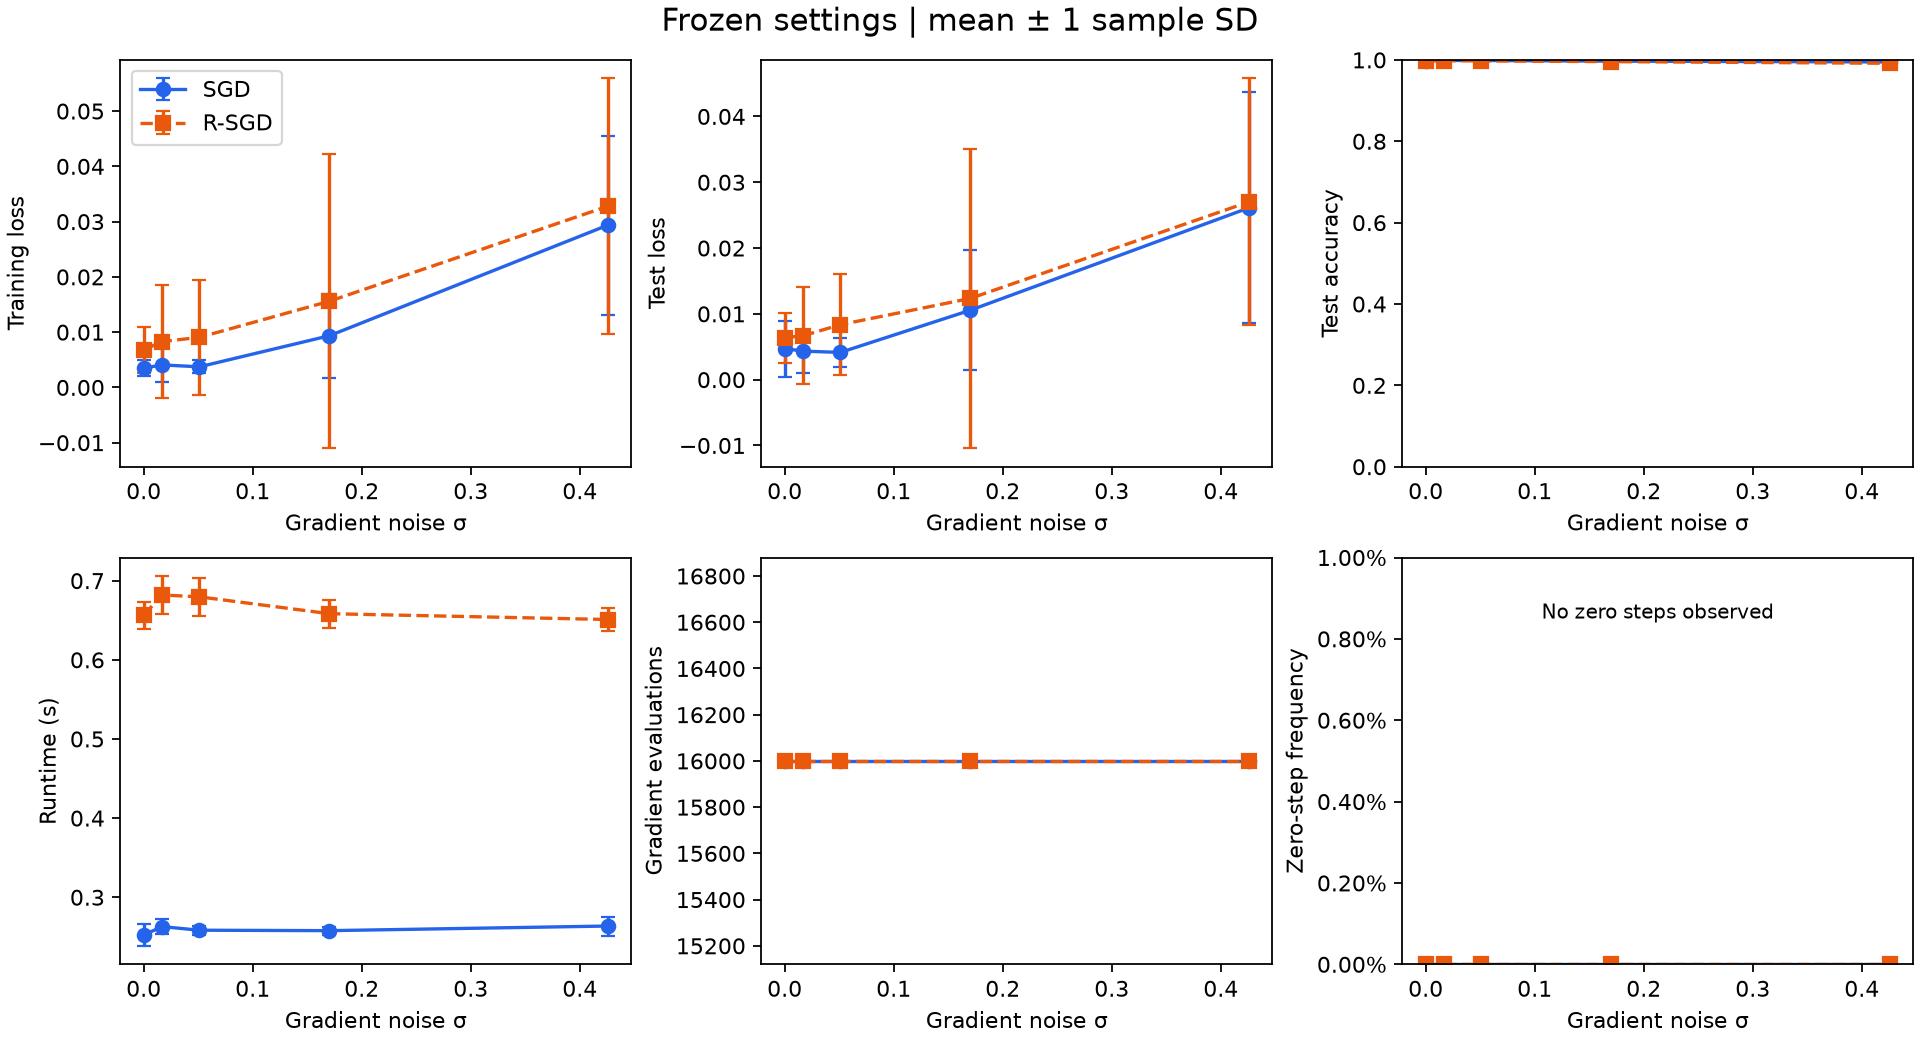
\includegraphics[width=\textwidth]{./plots/semicircle/noise_summary.png}
    \caption{Simulation 2 final metrics against gradient noise.
    Mean $\pm$ one sample SD across 15 seeds.
    Top row shows training BCE, test BCE, and test accuracy.
    Bottom row shows runtime, gradient observations, and zero-step frequency.}
    \label{fig:sim2_metrics}
\end{figure}

\begin{figure}[p]
    \centering
    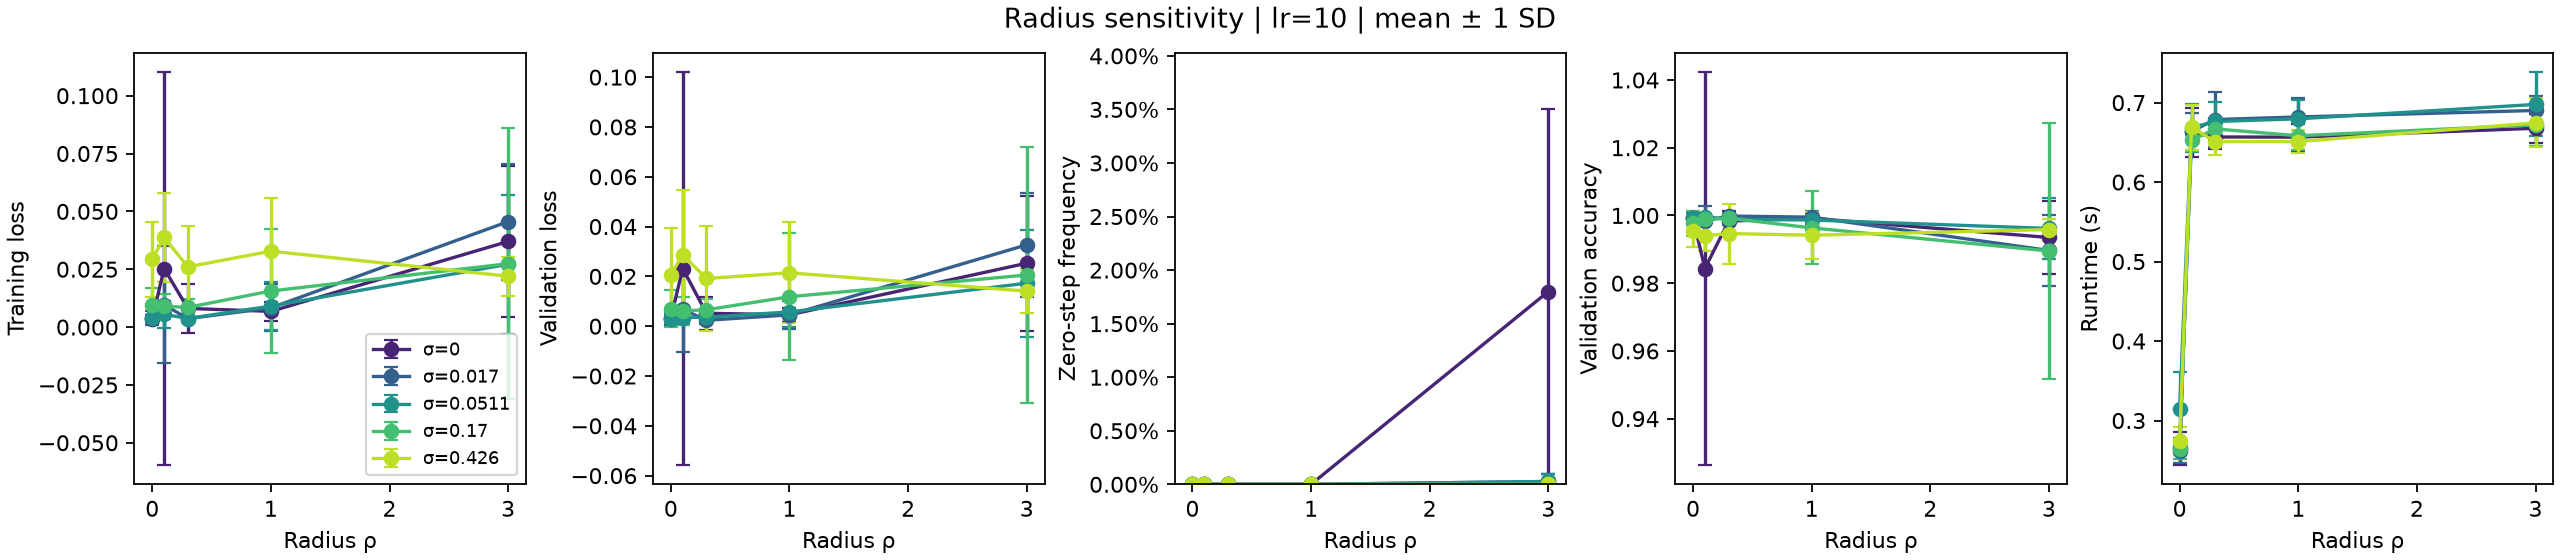
\includegraphics[width=\textwidth]{./plots/semicircle/radius_sensitivity.png}
    \caption{Simulation 2 radius sensitivity at LR 10.
    Panels show training loss, validation loss, zero-step frequency,
    validation accuracy, and full training-loop runtime.
    Every color denotes a gradient-noise level, with mean $\pm$ one sample SD
    across 15 seeds. The zero-step axis adapts to the observed frequency.}
    \label{fig:sim2_radius}
\end{figure}

\begin{figure}[p]
    \centering
    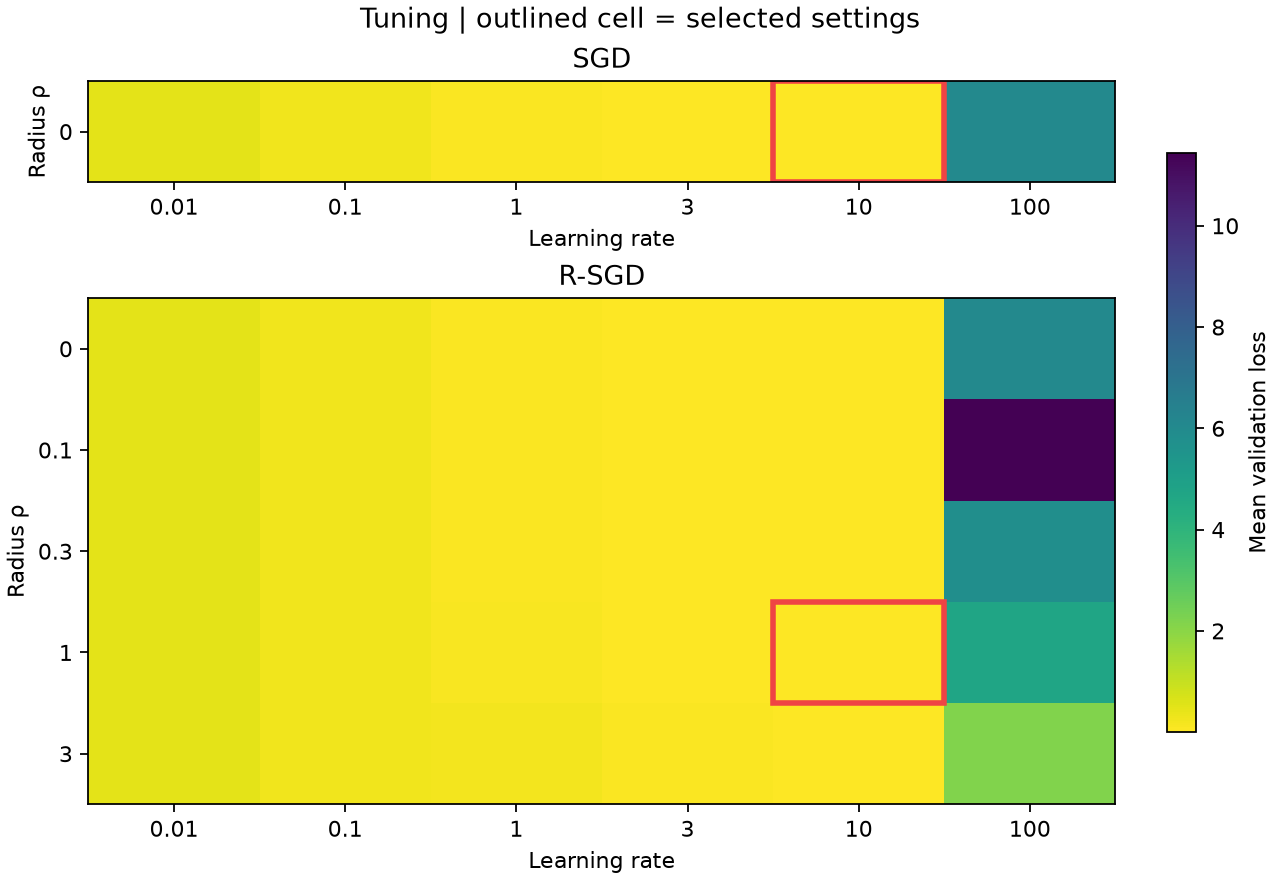
\includegraphics[width=0.9\textwidth]{./plots/semicircle/tuning.png}
    \caption{Simulation 2 clean validation-loss grid.
    Outlined cells show the selected SGD setting and the best positive-radius
    setting. The unrestricted robust-grid winner was radius zero.}
    \label{fig:sim2_tuning}
\end{figure}
\clearpage
